\documentclass[letterpaper]{article}
\usepackage[margin=1in]{geometry}
\usepackage[utf8]{inputenc}
\usepackage{textcomp}
\usepackage{amssymb}
\usepackage{natbib}
\usepackage{graphicx}
\usepackage{gensymb}
\usepackage{amsthm, amsmath, mathtools}
\usepackage[dvipsnames]{xcolor}
\usepackage{enumerate}
\usepackage{mdframed}
\usepackage[most]{tcolorbox}
\usepackage{csquotes}
% https://tex.stackexchange.com/questions/13506/how-to-continue-the-framed-text-box-on-multiple-pages

\tcbuselibrary{theorems}

\newcommand{\R}{\mathbb{R}}
\newcommand{\Z}{\mathbb{Z}}
\newcommand{\N}{\mathbb{N}}
\newcommand{\Q}{\mathbb{Q}}
\newcommand{\C}{\mathbb{C}}
\newcommand{\code}[1]{\texttt{#1}}
\newcommand{\mdiamond}{$\diamondsuit$}
\newcommand{\PowerSet}{\mathcal{P}}
\newcommand{\Mod}[1]{\ (\mathrm{mod}\ #1)}
\DeclareMathOperator{\lcm}{lcm}

%\newtheorem*{theorem}{Theorem}
%\newtheorem*{definition}{Definition}
%\newtheorem*{corollary}{Corollary}
%\newtheorem*{lemma}{Lemma}
\newtheorem*{proposition}{Proposition}


\newtcbtheorem[number within=section]{theorem}{Theorem}
{colback=green!5,colframe=green!35!black,fonttitle=\bfseries}{th}

\newtcbtheorem[number within=section]{definition}{Definition}
{colback=blue!5,colframe=blue!35!black,fonttitle=\bfseries}{def}

\newtcbtheorem[number within=section]{corollary}{Corollary}
{colback=yellow!5,colframe=yellow!35!black,fonttitle=\bfseries}{cor}

\newtcbtheorem[number within=section]{lemma}{Lemma}
{colback=red!5,colframe=red!35!black,fonttitle=\bfseries}{lem}

\newtcbtheorem[number within=section]{example}{Example}
{colback=white!5,colframe=white!35!black,fonttitle=\bfseries}{def}

\newtcbtheorem[number within=section]{note}{Important Note}{
        enhanced,
        sharp corners,
        attach boxed title to top left={
            xshift=-1mm,
            yshift=-5mm,
            yshifttext=-1mm
        },
        top=1.5em,
        colback=white,
        colframe=black,
        fonttitle=\bfseries,
        boxed title style={
            sharp corners,
            size=small,
            colback=red!75!black,
            colframe=red!75!black,
        } 
    }{impnote}
\usepackage[utf8]{inputenc}
\usepackage[english]{babel}
\usepackage{fancyhdr}
\usepackage[hidelinks]{hyperref}

\pagestyle{fancy}
\fancyhf{}
\rhead{CSE 101}
\chead{Friday, January 07, 2022}
\lhead{Lecture 3}
\rfoot{\thepage}

\setlength{\parindent}{0pt}

\begin{document}

\section{Graph Algorithm Runtimes}
Recall the following algorithms: 
\begin{verbatim}
    explore(v)
        v.visited = true 
        For each edge (v, w)
            If not w.visited
                explore(w)

    DepthFirstSearch(G)
        Mark all v in G as unvisited
        For v in G
            If not v.visited
                explore(v)
\end{verbatim}
Although $O(|V| + |E|)$ is linear time, in reality, graph algorithm runtimes depend on both $|V|$ and $|E|$. What algorithm is better may depend on the relative sizes of these parameters.

\begin{center}
    \begin{tabular}{c|c|c}
                & \textbf{Sparse Graphs} & \textbf{Dense Graphs} \\ 
        \hline
        Runtime & $|E|$ small ($\approx V$) & $|E|$ large ($\approx V^2$) \\ 
        Examples & Internet, Road Maps & Flight Maps, Wireless Networks 
    \end{tabular}
\end{center}

\section{Graph Representation}
How do you store a graph in a computer?
\begin{itemize}
    \item \textbf{Adjacency Matrix:} Store list of vertices and an array \code{A[i, j] = 1} if edge between $v_i$ and $v_j$.
    \begin{itemize}
        \item Slow space for dense graphs.
        \item Slow for most operations.
    \end{itemize}

    \item \textbf{Edge List:} List of all vertices with list of all edges. 
    \begin{itemize}
        \item More space-efficient for a sparse graph. 
        \item Hard to determine edges outof the single vertex.
    \end{itemize}

    \item \textbf{Adjacency List:} For each vertex, store a list of neighbors.
    \begin{itemize}
        \item Needed for DFS to be efficient. 
        \item We will usually assume this representation.
    \end{itemize}
\end{itemize}

\section{Connected Components}
We want to understand which vertices are reachable from which others in a graph. We've already kind of done this using \code{explore(v)} to find which vertices are reachable from a given vertex. 

\bigskip 

For a more theoretical answer, consider the theorem: 
\begin{theorem}{}{}
    The vertices of a graph $G$ can be partitioned into connected components so that $v$ is is reachable from $w$ if and only if they are in the same connected component. 
\end{theorem}

For instance, consider the following graph:
\begin{center}
    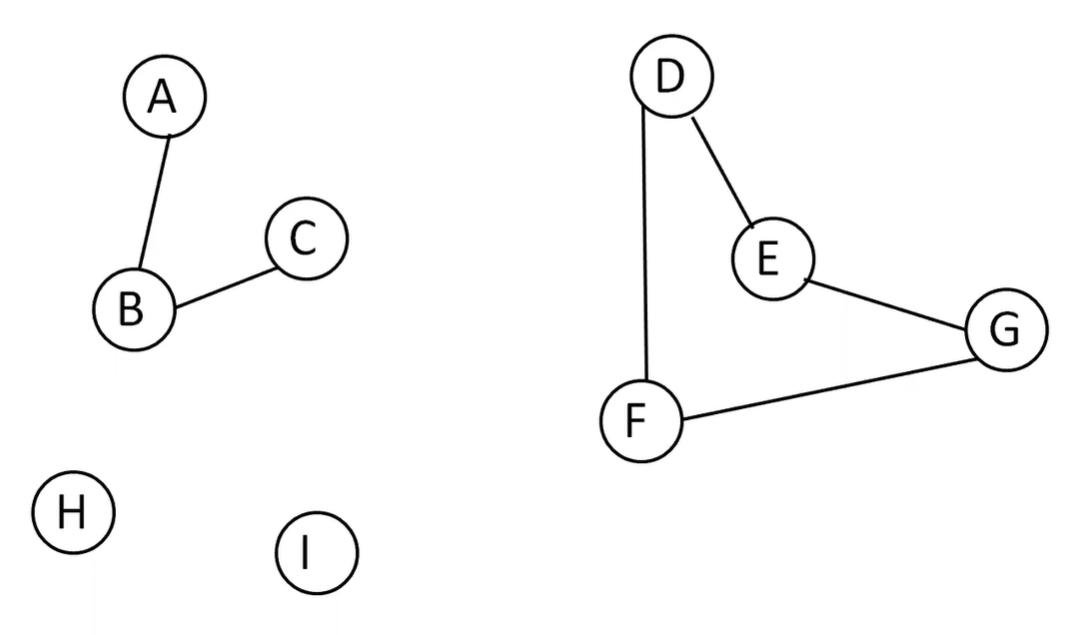
\includegraphics[scale=0.35]{../assets/graph_con.png}
\end{center}
We can split this graph into four components: 
\begin{center}
    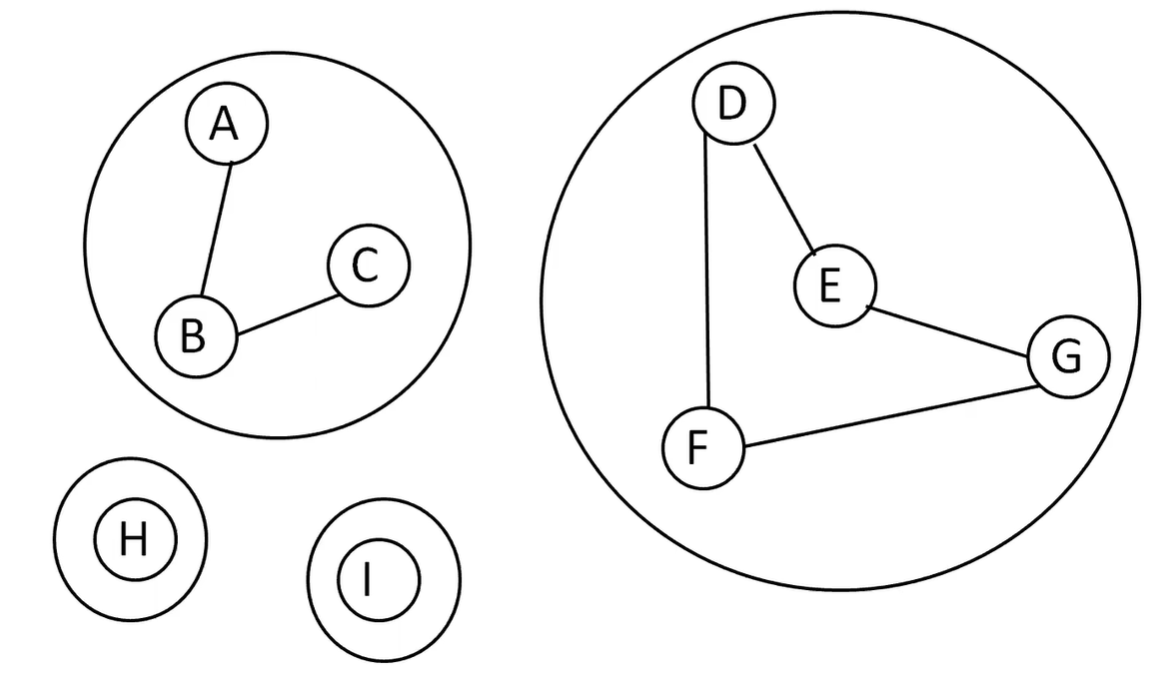
\includegraphics[scale=0.35]{../assets/graph_con_2.png}
\end{center}
Here, if there are two points in a component, then we can reach the first point from the second and vice versa. However, if there are two points in two different components, then this is not possible.  

\subsection{Computing Connected Components}
Given a graph $G$, how do we compute its connected components? 
\begin{itemize}
    \item \underline{Easy Way:} For each $v$, run \code{explore(v)} to find the vertices reachable from it. Group together into components. The runtime will be $O(|V|(|V| + |E|))$. 
    \item \underline{Better Way:} Run \code{explore(v)} to find the components of $v$. Then, repeat this on the unclassified vertices. 
\end{itemize}

\subsection{Applying Depth-First Search (DFS)}
We can use depth-first search to simulate this. In fact, we can use the same algorithm above but with a bit of additional ``information'' to get our answer:
\begin{verbatim}
    explore(v, CCNum):
        v.visited = true 
        // CC is connected components
        v.CC = CCNum 
        for each edge (v, w):
            if not w.visited: 
                explore(w)

    ConnectedComponents(G):
        CCNum = 0
        for each v in G:
            v.visited = false
        for each v in G: 
            if not v.visited: 
                CCNum++
                explore(v, CCNum)
\end{verbatim}
The runtime is $O(|V| + |E|)$. 

\bigskip

If we recall the graph above, running this algorithm would yield something like:
\begin{center}
    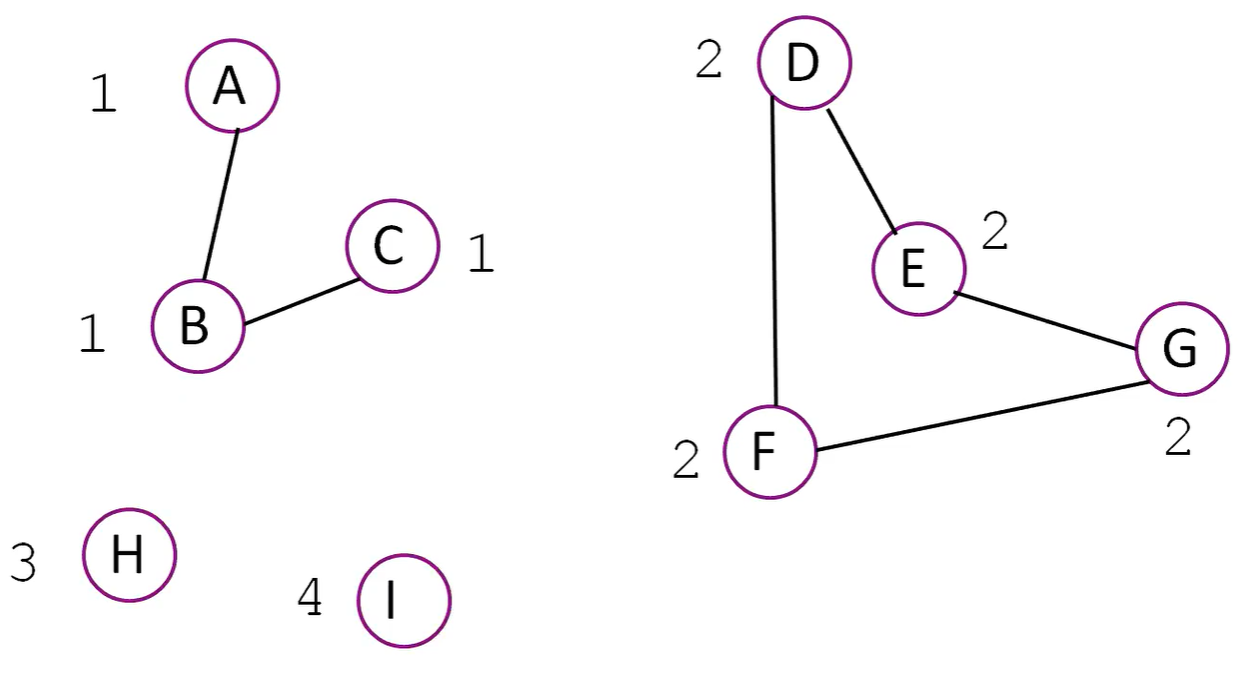
\includegraphics[scale=0.35]{../assets/graph_con_3.png}
\end{center}
Where \code{CCNum} is \code{4}, or 4 connected components. 


\subsection{DFS: A Discussion}
What does DFS actually do? 
\begin{itemize}
    \item No output.
    \item Marks all vertices as visited. 
    \item Easier ways to do it.
\end{itemize}
However, DFS is a useful way to \emph{explore the graph}. In particular, by augmenting the algorithm a bit, like we did with the connected components algorithm, we can learn useful things. In other words, DFS by itself is quite useless, but adding a bit of additional information will make it more useful. 

\subsection{Pre- and Post- Order}
How can we augment this algorithm?
\begin{itemize}
    \item Keep track of what algorithm does and in what order. 
    \item Have a ``clock'' and note time whenever: 
    \begin{itemize}
        \item Algorithm visits a new vertex for the first time. 
        \item Algorithm finishes processing a vertex.
    \end{itemize}
    \item Finally, we can record values as \code{v.pre} and \code{v.post}.
\end{itemize}

\subsection{Computing Pre- and Post- Order}
Consider the algorithm, which is the same thing as above but with some changes to make it useful: 
\begin{verbatim}
    explore(v)
        v.visited = true 
        v.pre = clock 
        clock++
        For each edge (v, w)
            If not w.visited
                explore(w)
        v.post = clock 
        clock++

    DepthFirstSearch(G)
        clock = 1
        Mark all v in G as unvisited
        For v in G
            If not v.visited
                explore(v)
\end{verbatim}
The runtime is still $O(|V| + |E|)$. 

\subsection{Example of Pre- and Post- Order}
Consider the following graph:
\begin{center}
    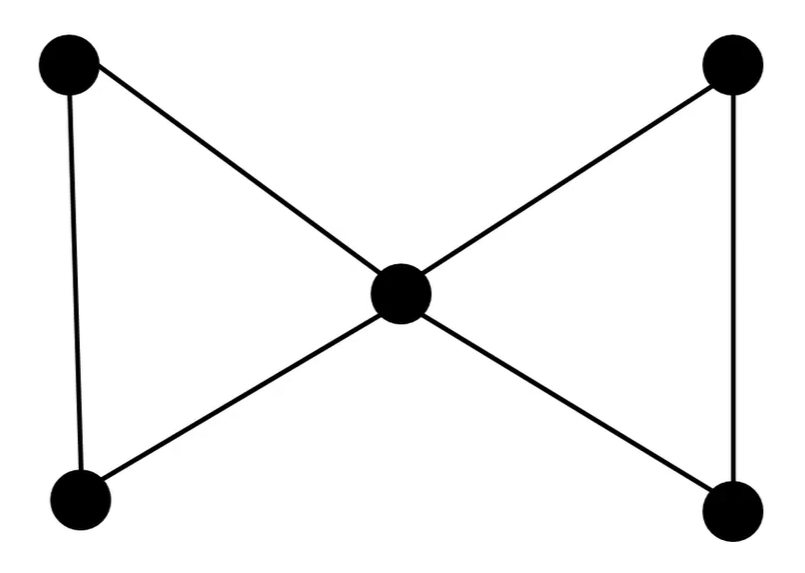
\includegraphics[scale=0.3]{../assets/graph_tri.png}
\end{center}
After running the above algorithm, we get:
\begin{center}
    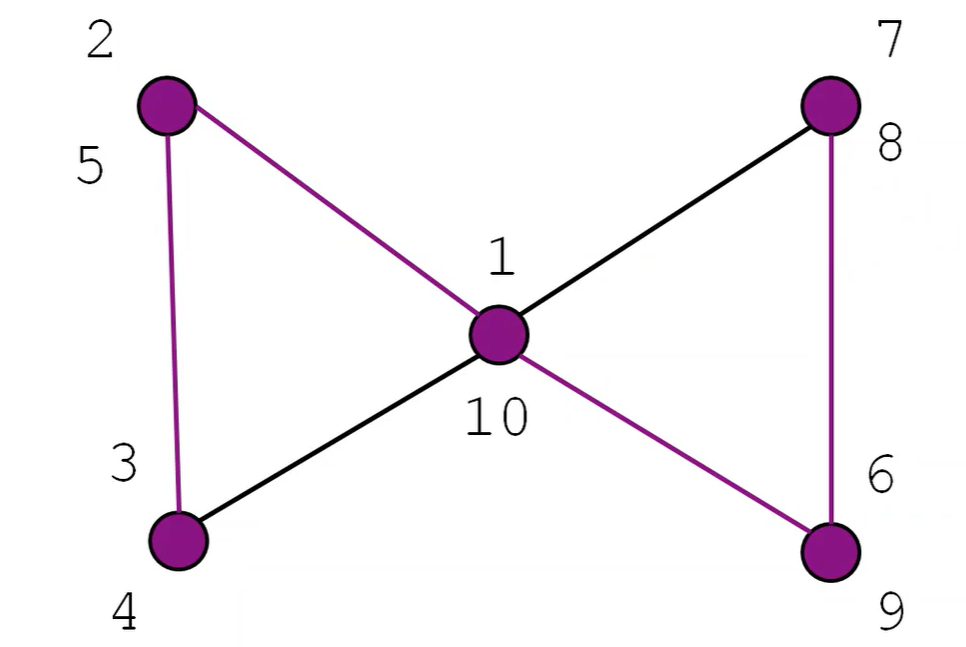
\includegraphics[scale=0.3]{../assets/graph_tri_2.png}
\end{center}
How did we get this? 
\begin{itemize}
    \item We assign \code{1} to the center vertex. \code{1} has an unexplored neighbor, which is the top-left vertex.
    \item We assign \code{2} to the top-left vertex. \code{2} has an unexplored neighbor, which is the bottom-left vertex. 
    \item We assign \code{3} to the bottom-left vertex. \code{3} doesn't have any other unexplored neighbors.  
    \item Since we can't go anywhere from \code{3}, we assign it a post-order value of \code{4}.
    \item Now that we're back at \code{2}, note that there aren't any other unexplored edges, so we give it a post-order value of \code{5}.
    \item We're now back at the center vertex. However, we still have more to explore.
    \item We assign \code{6} to the bottom-right vertex. 
    \item We assign \code{7} to the top-right vertex. 
    \item Since we can't go anywhere from \code{7}, we assign it a post-order value of \code{8}.
    \item Now that we're back at \code{6}, we assign it a post-order value of \code{9} since we can't explore anything else.
    \item Now that we're back at \code{1}, we assign it a post-order value of \code{10} since we can't explore anything else. 
\end{itemize}
If the graph is connected, the first vertex will always be the last vertex. However, if the graph is disconnected, the first vertex may not necessarily be the last vertex. 

\subsection{Application of Orders}
\begin{proposition}
    For vertices $v$, $w$, we can consider the intervals \code{[v.pre, v.post]} and \code{[w.pre, w.post]}. These intervals:
    \begin{enumerate}
        \item contain each other if $v$ is an ancestor/descendant of $w$ in the DFS tree. 
        \item are disjoint if $v$ and $w$ are cousins in the DFS tree.
        \item never interleave (\code{v.pre < w.pre < v.post < w.post}).
    \end{enumerate}
\end{proposition}

\begin{mdframed}[]
    \begin{proof}
        Assume that the algorithm finds $v$ before $w$ (\code{v.pre < w.pre}). If the algorithm discovers $w$ after fully processing $v$, then: 
        \begin{itemize}
            \item \code{v.post < w.pre}
            \item Intervals are disjoint 
            \item $v$ and $w$ are cousins.
        \end{itemize}
        If the algorithm discovers $w$ before fully processing $v$:
        \begin{itemize}
            \item The algorithm finishes processing $w$ before it finishes $v$.
            \item \code{v.pre < w.pre < w.post < v.post}
            \item Represents nested intervals. 
            \item $v$ is an ancestor of $w$. 
        \end{itemize}
        And so we are done.
    \end{proof}
\end{mdframed}

\section{Directed Graphs}
Often, an edge makes sense both ways. But, sometimes, streets are one directional.
\begin{definition}{}{}
    A \textbf{directed graph} is a graph where each edge has a direction. We say that it goes from $v$ to $w$. 
\end{definition}
Often, we draw arrows on the edges to denote direction. 

\subsection{DFS on Directed Graphs}
We can use DFS on a directed graph. However, we only follow directed edges from $v$ to $w$. The runtime is still $O(|V| + |E|)$, and \code{explore(v)} discovers all vertices reachable from $v$ following only directed edges. 

\end{document}